\documentclass[tikz,dvipdfmx]{jsarticle}

\usepackage{wrapfig}
\usepackage{graphicx}

\begin{document}
\begin{wrapfigure}[9]{l}[0mm]{45mm}
  \centering
  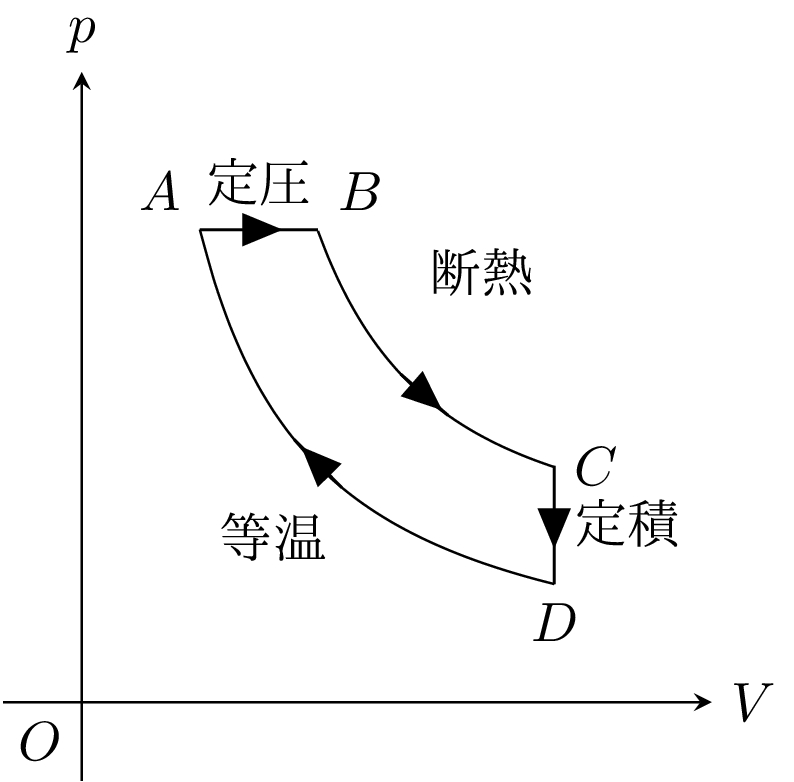
\includegraphics[keepaspectratio,width=45mm]{./req.png}
  \caption{}
  \label{graph}
\end{wrapfigure}

滑らかに動くピストンがついたシリンダー内に状態$A$の理\\
想気体がある.気体,外部間で熱,仕事のやりとりをして,気体\\
を状態変化させた.
以下の問に答えよ.ただし,$A \rightarrow B \rightarrow C \rightarrow \\
D \rightarrow A$と図1のように状態変化させている.\\ \\
$(1)$気体の内部エネルギーの変化が$0$になるのは,どの変化か.\\
$(2)$外部に正の仕事をするのは,どの変化か.\\
$(3)$気体が熱を外部に放出するのは,どの変化か.\\
$(4)$気体の温度が最低な状態は$A,B,C,D$のうちどの状態か.\\

\end{document}
